\documentclass{bioinfo}
\copyrightyear{2017} \pubyear{2017}

\access{Advance Access Publication Date: Day Month Year}
\appnotes{Manuscript Category}

\setcitestyle{square,sort,comma,numbers} 

\usepackage[colorlinks,
            linkcolor=blue,
            anchorcolor=blue,
            citecolor=blue,
			urlcolor=blue
            ]{hyperref}

\usepackage{url}
\usepackage{algorithm}
\usepackage{algorithmic}
\usepackage{color}
\newcommand{\comR}[1]{#1}
\newcommand{\comG}[1]{#1}
\newcommand{\comB}[1]{#1}
\newcommand{\comM}[1]{#1}
\newcommand{\comC}[1]{#1}
\begin{document}
\firstpage{1}

\subtitle{Subject Section}

\title[Bearing Fault Diagnosis Based on Deep Belief Network]{Bearing Fault Diagnosis Based on Deep Belief Network}
\author[Sun.]{Wujie Sun\,$^{\text{\sfb 1,}*}$}
\address{$^{\text{\sf 1}}$School of Software Engineering, South China University of Technology, Guangzhou 510006, P.R. China.}

\corresp{$^\ast$To whom correspondence should be addressed.}

\history{Received on XXXXX; revised on XXXXX; accepted on XXXXX}

\editor{Associate Editor: XXXXXXX}

\abstract{
It is important to judge whether the bearing is faulty and the possible fault location based on the acceleration of the bearing. However, the acceleration of the bearing is affected by noise, and it is difficult to rely on the observation to find the law. This problem can be solved by using wavelet packet decomposition and deep belief network. In this paper, we use wavelet packet decomposition for noise reduction, and extract features from the noise-reduced data, and then use the deep belief network (DBN) for training. The experimental results show its effectiveness.\\
\textbf{Keywords:} Deep belief network, fault diagnosis, wavelet packet decomposition, feature extraction\\
\textbf{Contact:} \href{mailto:wjsunscut@163.com}{wjsunscut@163.com}
}

\maketitle

\section{Introduction}
Mechanical bearing failures are common in daily life, and the economic and time loss they cause is very serious. Therefore, it is very important to find it early in the event of a failure. Accelerometer data collected from actual operating environment is an important indicator to determine whether the bearing is faulty. However, the acceleration of the bearing is affected by noise, and it is difficult to rely on observation to find the problem. Therefore, we need a method that can efficiently determine whether the bearing is faultly and its fault type by using the accelerometer data. 

Since the accelerometer data is affected by noise, we need to perform noise reduction. Wavelet packet decomposition \cite{Wang2015Detection}\cite{Yongle2015Zero} is widely used for noise reduction and has achieved remarkable results.


In recent years, deep learning, as an emerging method in the field of machine learning, has achieved brilliant results in the fields of image and speech recognition with its powerful capabilities. As one of the classical algorithms of deep learning, deep belief network \cite{Hinton2012A} successfully solves problems such as information retrieval, dimension reduction, fault classification and so on with its excellent feature extraction and training algorithms. The deep learning method has the following advantages compared with the traditional fault diagnosis methods: 1) Deep learning has powerful feature extraction ability, which can automatically extract features from a large amount of data, and reduces the needs of the expert experience and signal processing technology. It reduces the uncertainty of feature extraction and fault diagnosis caused by human in traditional methods; 2) By establishing a deep model, it can well represent the complex mapping relationship between signal and health status, which is very suitable for big data background. The need for diagnostic analysis of diverse, nonlinear, and high-dimensional health monitoring data. Therefore, applying deep learning to the field of fault diagnosis has certain timeliness, practicability and versatility.

In addition, deep belief network has better scalability and mapping capabilities than other machine learning algorithms such as support vector machine \cite{vapnik1999overview} and back propagation neural network \cite{Kramer1990Diagnosis}.

For the input data of the deep belief network, some choose to use the time domain signal as the input \cite{guangquan2016fault}, and some choose to use the frequency domain signal as the input \cite{jia2016deep}. In this paper, we choose to extract features from the time domain and the frequency domain as the input to the deep belief network \cite{YiThe}. Documents can be found on \href{https://github.com/wjsunscut/Intelligent-Software-Project-Training}{https://github.com/wjsunscut/Intelligent-Software-Project-Training}.

\section{Wavelet Packet Decomposition and Feature Extraction}
Wavelet packet decomposition uses an analysis tree to represent wavelet packets, that is, using multiple iterations of wavelet transform to analyze the details of the input signal. From the perspective of function theory, wavelet packet decomposition is to map the signal into the space formed by the wavelet packet basis function. From the perspective of signal processing, it is to pass the signal through a series of filters with different center frequencies but the same bandwidth.

Since the wavelet decomposition \cite{Walczak1997Noise} is poor in frequency resolution in the high frequency band and time resolution in the low frequency band, wavelet packet is proposed to overcome this problem. It is a more sophisticated method of signal analysis that improves the time domain resolution of the signal. Fig. \ref{fig:wpd} shows the difference between them.

\begin{figure}[htbp]
	\centering
	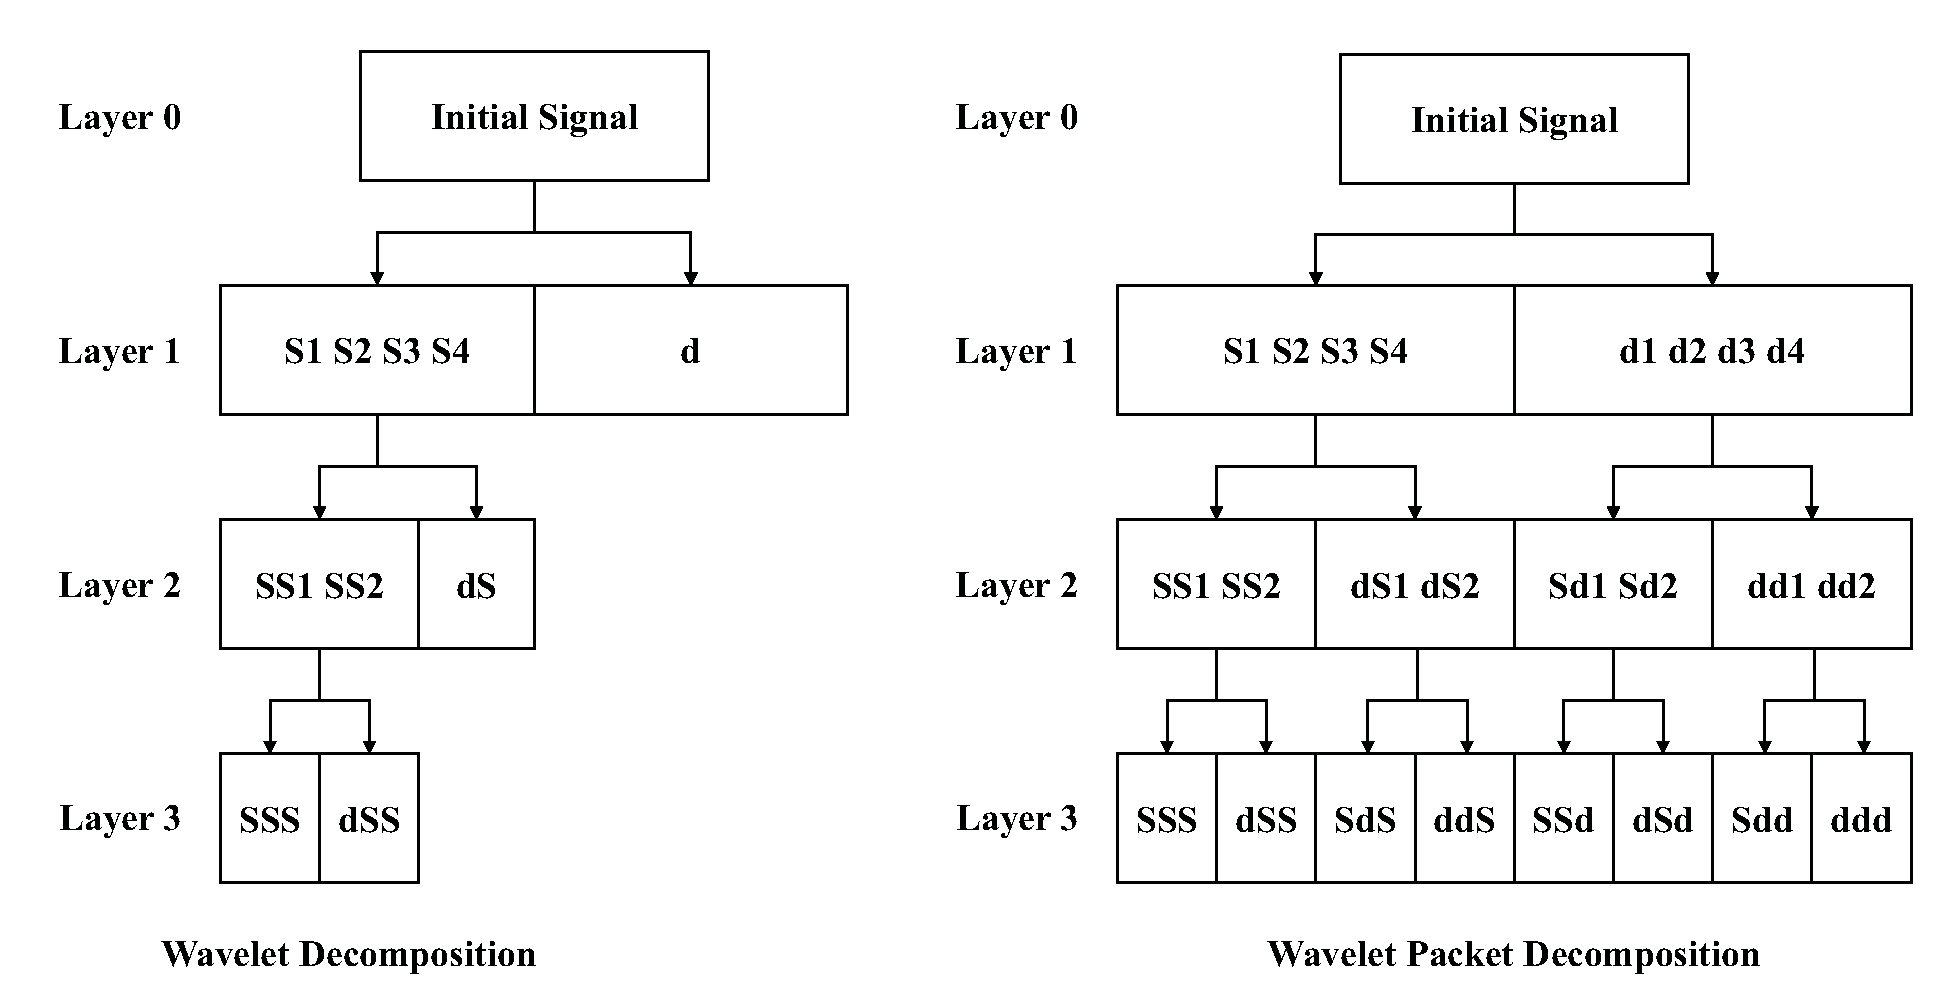
\includegraphics[width=\columnwidth]{wpd.eps}
	\caption{Difference between wavelet decomposition and wavelet packet decomposition.}
	\label{fig:wpd}
\end{figure}

Since wavelet packet decomposition is not the main content of this article, it is not described too much. Wavelet packet decomposition can be easily implemented using functions such as wavedec, appcoef, detcoef, wbmpen, and wdencmp in MATLAB (The specific code associated with the wavelet packet decomposition is in $preprocessing.m$ in the $Code$ folder).

Through the wavelet packet decomposition, we obtained the noise-reduced data. Next, we should extract features from the data. We need to set a sliding window to read the data by its length. For example, if there are 50,000 data and the sliding window length is 1000 and the number of statistical features is 100, then we can get 50 data with each containing 100 parameters. Table \ref{tab:sf} shows how to calculate the statistical features. $N$ is the length of sliding window and $x_i$ is the $i^{th}$ accelerometer data in the sliding window. More discriminating parameters can help to improve the accuracy of the classification. Limited to the paper space, we only provide 18 statistical features related to the time domain in the paper.

\begin{table}[htbp]
	\centering
	\caption{Statistical Features}  
	\begin{tabular}{|c|c|}  
		\hline  
		Name & Formula\\  
		\hline  
		Peak-to-Peak  & $\mathrm{M} \mathrm{AX}|x_i|-\mathrm{MIN}|x_i|$ \\
		\hline  
		Peak  & $\mathrm{M} \mathrm{A} \mathrm{X}|x_i|$ \\ 
		\hline  
		Mean  & $\frac{1}{N} \sum\limits_{i}^{N} x_i$ \\ 
		\hline  
		Mean Square  & $\frac{1}{N} \sum\limits_{i}^{N} x_i^{2}$ \\ 
		\hline  
		Root Mean Square  & $\sqrt{\frac{1}{N} \sum\limits_{i}^{N} x_i^{2}}$ \\ 
		\hline  
		Mean Amplitude  & $\frac{1}{N} \sum\limits_{i}^{N}|x_i|$ \\
		\hline  
		Square Mean Root  & $\left(\frac{1}{N} \sum\limits_{i}^{N}|x_i|^{1 / 2}\right)^{2}$ \\ 
		\hline  
		Variance  & $\frac{1}{N} \sum\limits_{i}^{N}(x_i-\overline{x})^{2}$ \\ 
		\hline  
		Standard Deviation  & $\sqrt{\frac{1}{N} \sum\limits_{i}^{N}(x_i-\overline{x})^{2}}$ \\
		\hline   
		Skewness  & $\frac{1}{N} \sum\limits_{i}^{N} x_i^{3}$ \\ 
		\hline  
		Kurtosis  & $\frac{1}{N} \sum\limits_{i}^{N}|x_i|^{4}$ \\
		\hline  
		Skewness Factor  & $\frac{1}{N} \sum\limits_{i}^{N}|x_i|^{3} /\left(\sqrt{\frac{1}{N} \sum\limits_{i}^{N} x_i^{2}}\right)^{3}$ \\ 
		\hline  
		Kurtosis Factor  & $\frac{1}{N} \sum\limits_{i}^{N}|x_i|^{4} /\left(\sqrt{\frac{1}{N} \sum\limits_{i}^{N} x_i^{2}}\right)^{4}$ \\ 
		\hline  
		Peak Factor  & $\mathrm{MAX}|x_i| / \sqrt{\frac{1}{N} \sum\limits_{i}^{N} x_i^{2}}$ \\ 
		\hline  
		Impulsive Factor  & $\operatorname{MAX}|x_i| / \frac{1}{N} \sum\limits_{i}^{N}|x_i|$ \\ 
		\hline  
		Clearance Factor  & $\operatorname{MAX}|x_i| /\left(\frac{1}{N} \sum\limits_{i}^{N}|x_i|^{1 / 2}\right)^{2}$ \\ 
		\hline  
		Waveform Factor  & $\sqrt{\frac{1}{N} \sum\limits_{i}^{N} x_i^{2}} / \frac{1}{N} \sum\limits_{i}^{N}|x_i|$ \\ 
		\hline  
		Waveform Entropy \cite{ZHANG201914} & $\frac{1}{N}\sum\limits_{i}^{N}x_i\log x_i$ \\ 
		\hline  
	\end{tabular} 
	\label{tab:sf} 
\end{table} 

\section{Deep Belief Network}
A common DBN model \cite{hinton2006fast} proposed by Hinton consists of a classifier and multiple restricted Boltzmann machines (RBMs) as shown in Fig. \ref{fig:dbn}. If we want to figure out the principles of the DBN, first we need to master the knowledge related to RBM.

\begin{figure}[htbp]
	\centering
	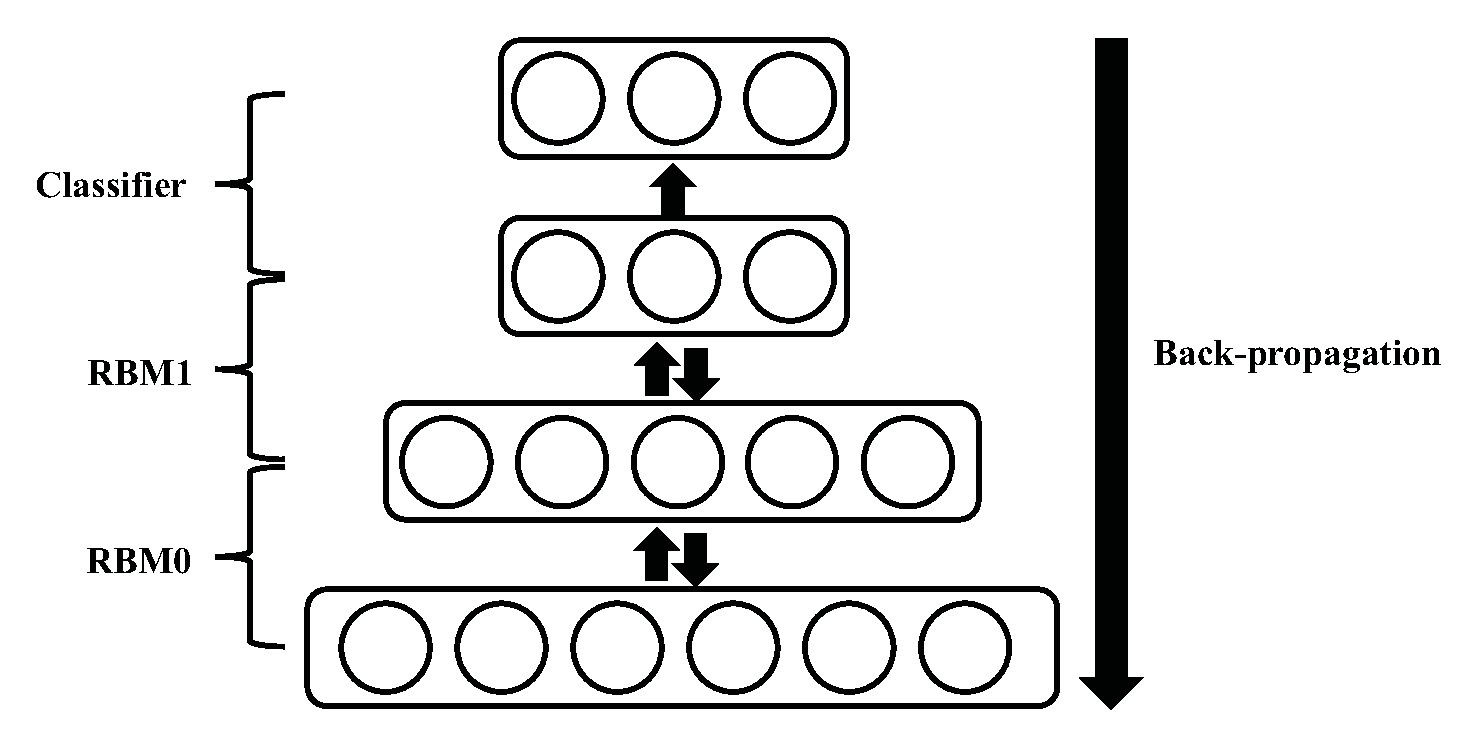
\includegraphics[width=\columnwidth]{dbn.eps}
	\caption{A simple DBN model with two RBMs and one classifier.}
	\label{fig:dbn}
\end{figure}

\subsection{Restricted Boltzmann Machine}
RBM \cite{hinton1986learning} has a visible layer, a hidden layer, but there is no connection within the layer, and is fully connected between the layers. And each layer unit takes a value of 0 or 1. It removes the intra-layer connection of the Boltzmann machine (BM), which greatly reduces the amount of calculation. The structure of the RBM is shown in Fig. \ref{fig:rbm}.
		
\begin{figure}[htbp]
	\centering
	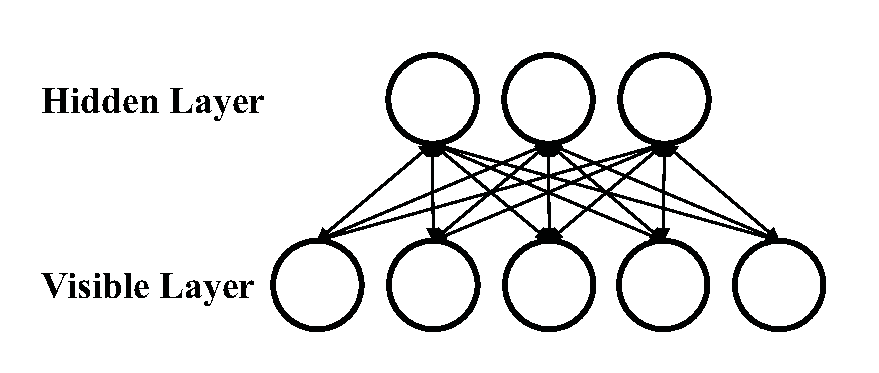
\includegraphics[width=\columnwidth]{rbm.eps}
	\caption{A simple RBM model with three hidden layer units and five visible layer units.}
	\label{fig:rbm}
\end{figure}
	
In RBM, the activation conditions of each hidden layer units are independent when the visible layer units' state is given. Similarly, the activation conditions of the visible layer units are independent when the hidden layer units' state is given.

The essence of RBM is a useful tool for unsupervised learning, which can be used for dimensionality reduction, feature extraction, autoencoder, deep belief network, and so on.

Next we will formulate the formula according to \cite{zhangchunxia}. Assume the RBM has $n$ visible layer units and $m$ hidden layer units. We use the vectors $\mathbf{v}$ and $\mathbf{h}$ to represent the states of its visible layer and hidden layer where $v_i$ is the $i^{th}$ visible layer unit and $h_j$ is the $j^{th}$ hidden layer unit. Therefore, for a given state $(\mathbf{v}, \mathbf{h})$, the energy of the RBM can be calculated as
\begin{equation}
E(\mathbf{v}, \mathbf{h})=-\sum_{i=1}^{m} \sum_{j=1}^{n} w_{i j} v_{i} h_{j}-\sum_{i=1}^{m} a_{i} v_{i}-\sum_{j=1}^{n} b_{j} h_{j}
\end{equation}
where $w_{ij}$ is the weight, $a_{i}$ is the visible layer unit bias, $b_{j}$ is the hidden layer unit bias, and $\boldsymbol{\theta}=\{w_{ij}, a_i, b_j\}$.

After that, the joint probability distribution can be calculated as 
\begin{equation}
P(\mathbf{v}, \mathbf{h} | \boldsymbol{\theta})=\frac{\mathbf{e}^{-E(\mathbf{v}, \mathbf{h} | \boldsymbol{\theta})}}{Z(\boldsymbol{\theta})}, \quad Z(\boldsymbol{\theta})=\sum_{\mathbf{v}, \mathbf{h}} \mathrm{e}^{-E(\mathbf{v}, \mathbf{h} | \boldsymbol{\theta})}
\end{equation}
and the likehood function can be calculated as
\begin{equation}
P(\mathbf{v} | \boldsymbol{\theta})=\frac{1}{Z(\boldsymbol{\theta})} \sum_{\mathbf{h}} \mathrm{e}^{-E(\mathbf{v}, \mathbf{h} | \boldsymbol{\theta})}
\end{equation}

By formula derivation, we can get the following activation probability formula
\begin{equation}
P\left(h_{j}=1 | \mathbf{v}, \boldsymbol{\theta}\right)=\sigma\left(b_{j}+\sum_{i} v_{i} w_{i j}\right)
\end{equation}
\begin{equation}
P\left(v_{i}=1 | \mathbf{h}, \boldsymbol{\theta}\right)=\sigma\left(a_{i}+\sum_{j} w_{i j} h_{j}\right)
\end{equation}
where $\sigma(x)=1/(1+e^{-x})$.
\subsection{Contrastive Divergence Algorithm}
The purpose of using RBM is to find the suitable value of $\boldsymbol{\theta}$ to fit the given training data. However, obtaining results based on methods such as Gibbs sampling is cumbersome and time consuming \cite{zhangchunxia}. Fortunately, Hinton proposed an algorithm called Contrastive Divergence (CD) \cite{Hinton2002Training} which is easy to calculate. Algorithm is shown as Alg. \ref{alg:cd}. By using the CD algorithm, the suitable $\boldsymbol{\theta}$ value can be calculated very conveniently and quickly.
\begin{algorithm}
	\caption{Contrastive Divergence}
	\label{alg:cd}
	\begin{algorithmic}[1]
		\STATE Training sample $x_0$, learning rate $\epsilon$, max epoch $T$;
		\STATE $\mathbf{v_1}=x_0$, $\mathbf{w}$, $\mathbf{a}$, and $\mathbf{b}$ are random small values;
		\FOR{$epoch = 1,2,...,T$}
		\FOR{$j=1,2,...,m$}
			\STATE Calc $P\left(h_{1j}=1 | \mathbf{v_1} \right)=\sigma\left(b_{j}+\sum_{i} v_{1i} w_{i j}\right)$;
			\STATE Randomly select $h_{1j}\in\{0,1\}$;
		\ENDFOR
		\FOR{$i=1,2,...,n$}
			\STATE Calc $P\left(v_{2i}=1 | \mathbf{h_1} \right)=\sigma\left(a_{i}+\sum_{j} h_{1j} w_{i j}\right)$;
			\STATE Randomly select $v_{2i}\in\{0,1\}$;
		\ENDFOR
		\FOR{$j=1,2,...,m$}
			\STATE Calc $P\left(h_{2j}=1 | \mathbf{v_2} \right)=\sigma\left(b_{j}+\sum_{i} v_{2i} w_{i j}\right)$;
		\ENDFOR
		\STATE $\mathbf{\triangle w}=P(h_{1.}=1|\mathbf{v_1})\mathbf{v_1^T}-P(h_{2.}=1|\mathbf{v_2})\mathbf{v_2^T}$;
		\STATE $\mathbf{\triangle a}=\mathbf{v_1}-\mathbf{v_2}$;
		\STATE $\mathbf{\triangle b}=P(h_{1.}=1|\mathbf{v_1})-P(h_{2.}=1|\mathbf{v_2})$;
		\STATE $\mathbf{w}\leftarrow \mathbf{w}+\epsilon\triangle\mathbf{w}$;
		\STATE $\mathbf{a}\leftarrow \mathbf{a}+\epsilon\triangle\mathbf{a}$;
		\STATE $\mathbf{b}\leftarrow \mathbf{b}+\epsilon\triangle\mathbf{b}$;
		\ENDFOR
	\end{algorithmic} 
\end{algorithm} 
\subsection{Train DBN}
Now we construct DBN as shown in Fig. \ref{fig:dbn}. First, we input the data into RBM0 and run CD algorithm. Then we should consider the output of RBM0 as the input of RBM1 and run CD algorithm. After that, we can see the whole network as back propagation neural network and train it. The $\boldsymbol{\theta}$ trained by RBMs should be the initial value of the back propagation neural network.

So what is the advantage of DBN compared to the traditional back propagation neural network? One problem with traditional multi-layer perception or neural network is that the back propagation may always result in local minima. Because when the error surface contains multiple grooves, the deepest groove may cannot be found when using the gradient descent. The deep belief network can solve the problem of local minimum through additional pre-training, i.e. RBM. Pre-training is done before back propagation so that the optimal point is not so far from the initial point. Then we can slowly approach the optimal point through back propagation.

\begin{figure}[htbp]
	\centering
	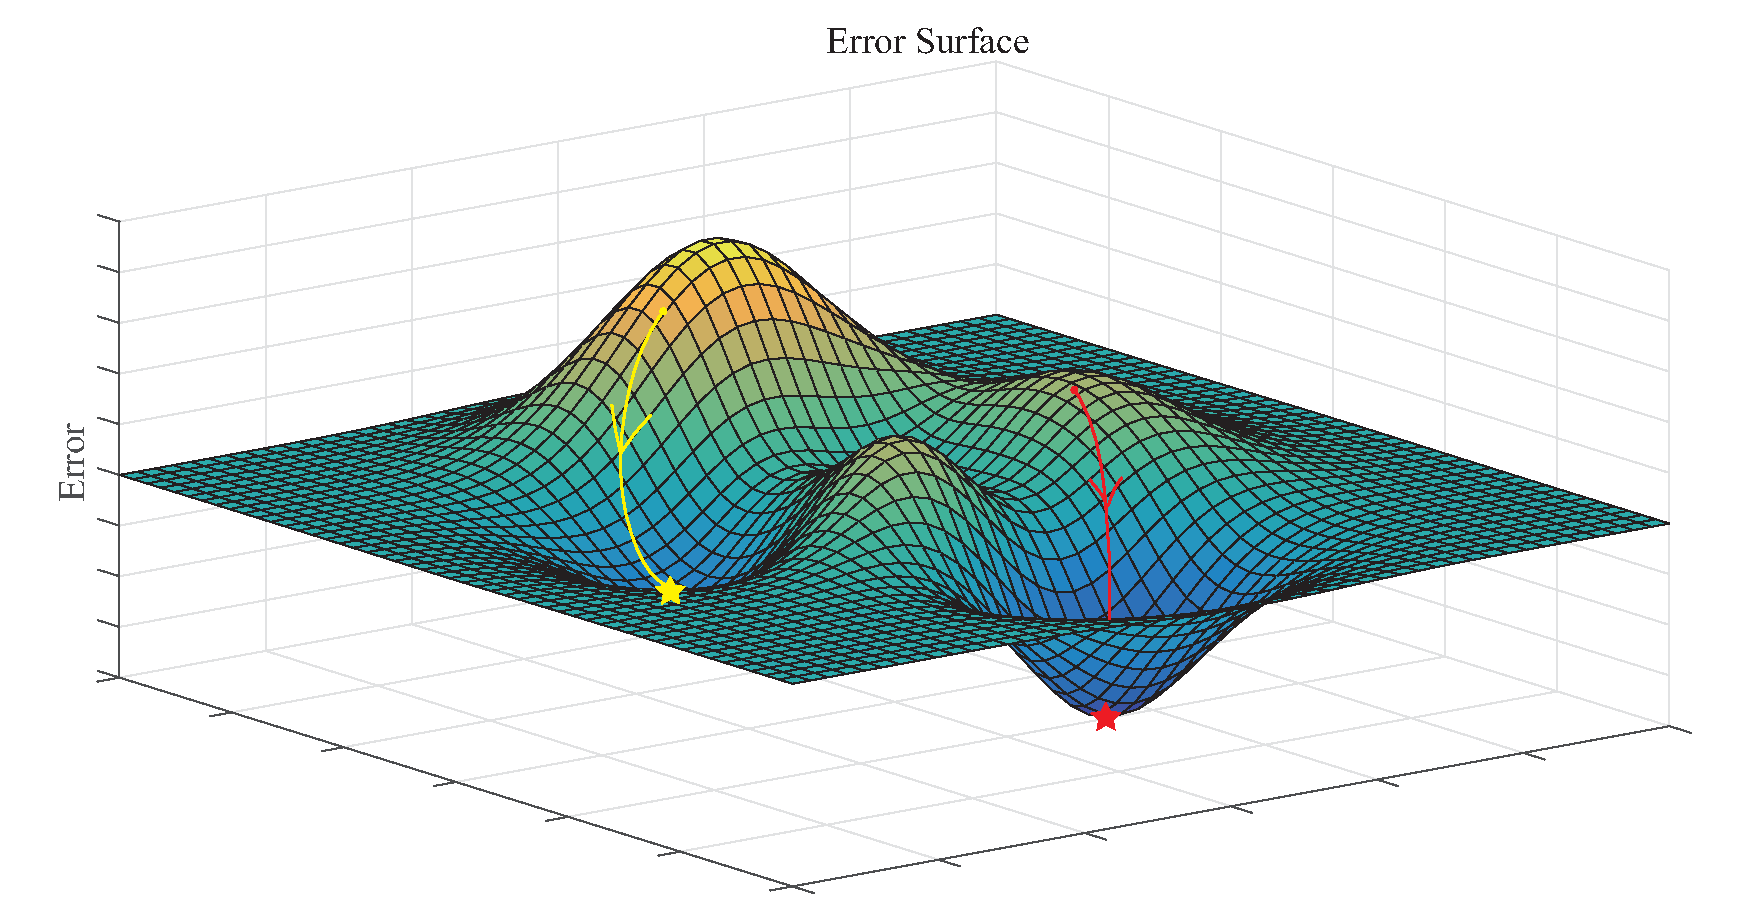
\includegraphics[width=\columnwidth]{surface.eps}
	\caption{Error surface with multiple grooves. The yellow pentagram indicates the local minimum point, and the red pentagram indicates the global minimum point. The yellow dot indicates the starting point when RBM is not used. The red dot indicates the starting point when RBM is used. The yellow and red curves indicate the gradient descent route. Obviously, the red starting point is more helpful for training to get a better classification model.}
	\label{fig:surface}
\end{figure}

This is the most basic DBN model and we can optimize it for better classification accuracy and performance. In \cite{YiThe}, the authors improved the activation function by combining Sigmoid with LReL to achieve the goal. Authors of \cite{wang2017improved} proposed the semi-supervised DBN (SSDBN) to improve the structure of the DBN to achieve better performance.

\textcolor{red}{In this project training, I reproduced these two papers. Since there is no suitable optimization method at present, in the DBN and experiment part, only the optimization methods of the published papers are involved. In addition, I found some problems in the process of reading and reproducing the papers, which I will explain and correct below.}
\subsection{Correction of Problems}
The $15^{th}$ formula in \cite{YiThe} is written incorrectly and should be changed to

\begin{equation}
\nonumber
f_{I}(x)=\left\{\begin{array}{ll}{\alpha(x-a)+\operatorname{Sigmoid}(a)} & {x>=a} \\ {\operatorname{Sigmoid}(x)} & {-a<x<a} \\ {\alpha(x+a)+\operatorname{Sigmoid}(-a)} & {x<=-a}\end{array}\right.
\end{equation}

The $17^{th}$ formula in \cite{wang2017improved} is written incorrectly and should be changed to
\begin{equation}
\nonumber
\begin{aligned} E(\boldsymbol{v}, \boldsymbol{u}, \boldsymbol{h} / \boldsymbol{\psi})=&-\sum_{i=1}^{m} a_{i} v_{i}-\sum_{j=1}^{n} b_{j} h_{j}-\sum_{i=1}^{m} \sum_{j=1}^{n} v_{i} w_{i j} h_{j} \\ &-\lambda \sum_{k=1}^{m} c_{k} u_{k}-\lambda \sum_{k=1}^{m} \sum_{j=1}^{n} u_{k} p_{k j} h_{j} \end{aligned}
\end{equation}
and the $18^{th}$ should be changed to
\begin{equation}
\nonumber
P\left(h_{j} / \boldsymbol{v}, \boldsymbol{u}, \psi\right)=\sigma\left(\sum_{i=1}^{m} v_{i} w_{i j}+\lambda \sum_{k}^{m} u_{k}p_{kj}+b_{j}\right)
\end{equation}

In addition, the corresponding derivatives are not given in the paper, so we give the results here. The specific derivation process is in the report.
\begin{equation}
\begin{aligned} 
\frac{\partial \log P(\boldsymbol{v}, \boldsymbol{u}, \boldsymbol{h})}{\partial w_{ij}}=&P(h_j=1|\boldsymbol{v^{(0)}},\boldsymbol{u^{(0)}})v_i^{(0)}\\&-P(h_j=1|\boldsymbol{v^{(1)}},\boldsymbol{u^{(1)}})v_i^{(1)}
\end{aligned}
\end{equation}

\begin{equation}
\begin{aligned} 
\frac{\partial \log P(\boldsymbol{v}, \boldsymbol{u}, \boldsymbol{h})}{\partial p_{kj}}=&\lambda P(h_j=1|\boldsymbol{v^{(0)}},\boldsymbol{u^{(0)}})u_k^{(0)}\\&-\lambda P(h_j=1|\boldsymbol{v^{(1)}},\boldsymbol{u^{(1)}})u_k^{(1)}
\end{aligned}
\end{equation}

\begin{equation}
\frac{\partial \log P(\boldsymbol{v}, \boldsymbol{u}, \boldsymbol{h})}{\partial a_{i}}=v_i^{(0)}-v_i^{(1)}
\end{equation}

\begin{equation}
\frac{\partial \log P(\boldsymbol{v}, \boldsymbol{u}, \boldsymbol{h})}{\partial c_{k}}=\lambda u_k^{(0)}-\lambda u_k^{(1)}
\end{equation}

\begin{equation}
\begin{aligned} 
\frac{\partial \log P(\boldsymbol{v}, \boldsymbol{u}, \boldsymbol{h})}{\partial b_{j}}=&P(h_j=1|\boldsymbol{v^{(0)}},\boldsymbol{u^{(0)}})\\&-P(h_j=1|\boldsymbol{v^{(1)}},\boldsymbol{u^{(1)}})
\end{aligned}
\end{equation}

\section{Experiments}
In the experiments in this paper, we used the drive end bearing accelerometer data provided by the Electrical Engineering Laboratory of Case Western Reserve University \cite{data}. \textcolor{red}{Since the content only covers the reproducing part, the main goal is to compare whether the various methods speed up the convergence or improve the classification accuracy rate when the parameters are basically consistent, instead of finding the highest classification accuracy rate.}

In the classification of faults, we refer to \cite{guangquan2016fault} to classify faults into 10 categories. In this experiment, 1500 data were used, that is, 150 data per category, and each data was extracted from 2048 continuous points to form statistical features.

First we use MATLAB to denoise the data, and the waveform comparison before and after noise reduction is shown in the Fig. \ref{fig:pre}. As we can see, by noise reduction, a large amount of noise is filtered out so that features can be more easily resolved.

\begin{figure}[htbp]
	\centering
	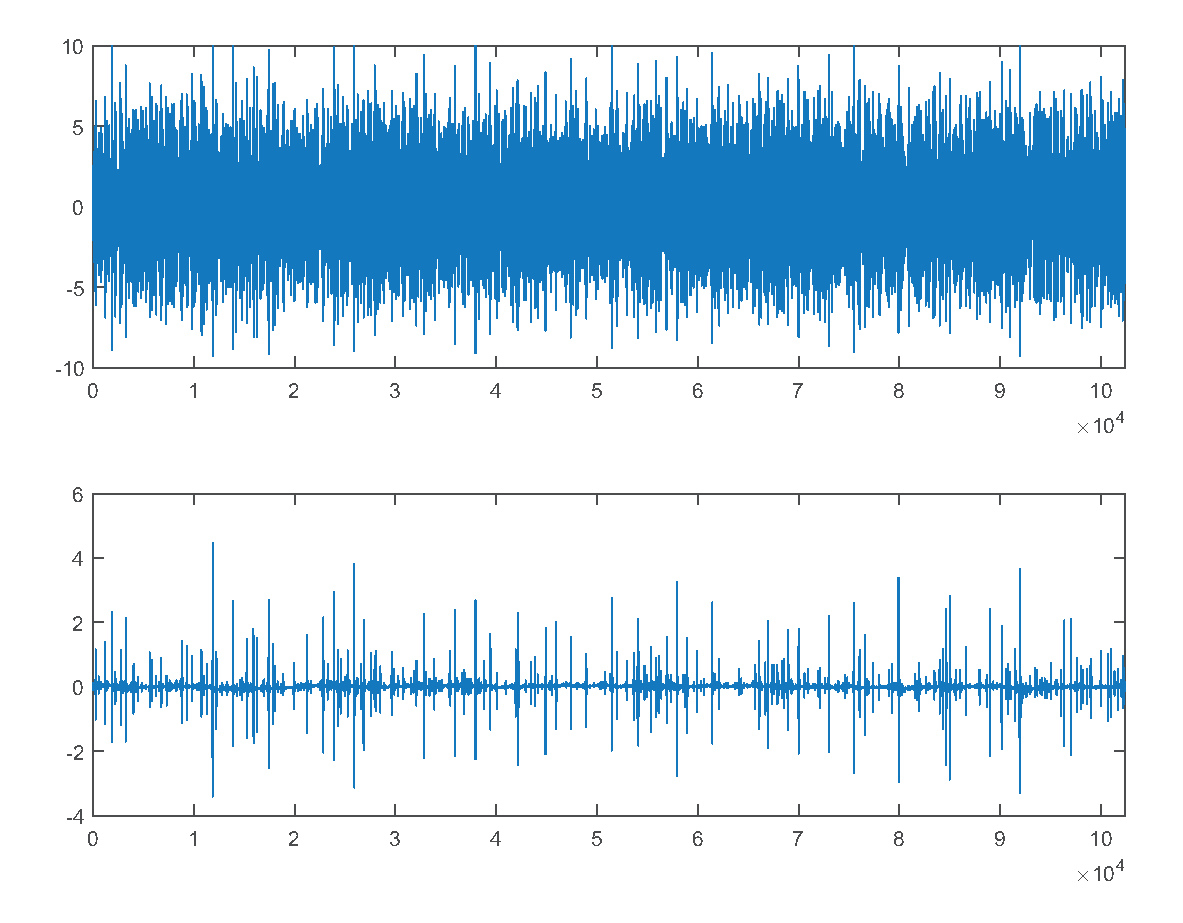
\includegraphics[width=\columnwidth]{pre.eps}
	\caption{The above figure is the original data, and the figure below is the data after noise reduction.}
	\label{fig:pre}
\end{figure}

Then we use the sliding window to segment the noise-reduced data and calculate its features according to Table \ref{tab:sf}. During the experiment, we found that noise reduction has the potential to remove useful signals, so when calculating features, we separately calculate the features of the original data and the noise-reduced data, and combine them together. The feature distribution can be seen in Fig. \ref{fig:feature}. It can be seen that different fault types have distinct feature distributions, so we should extract and use features which can distinguish different fault types easily and classify them.

\begin{figure}[htbp]
	\centering
	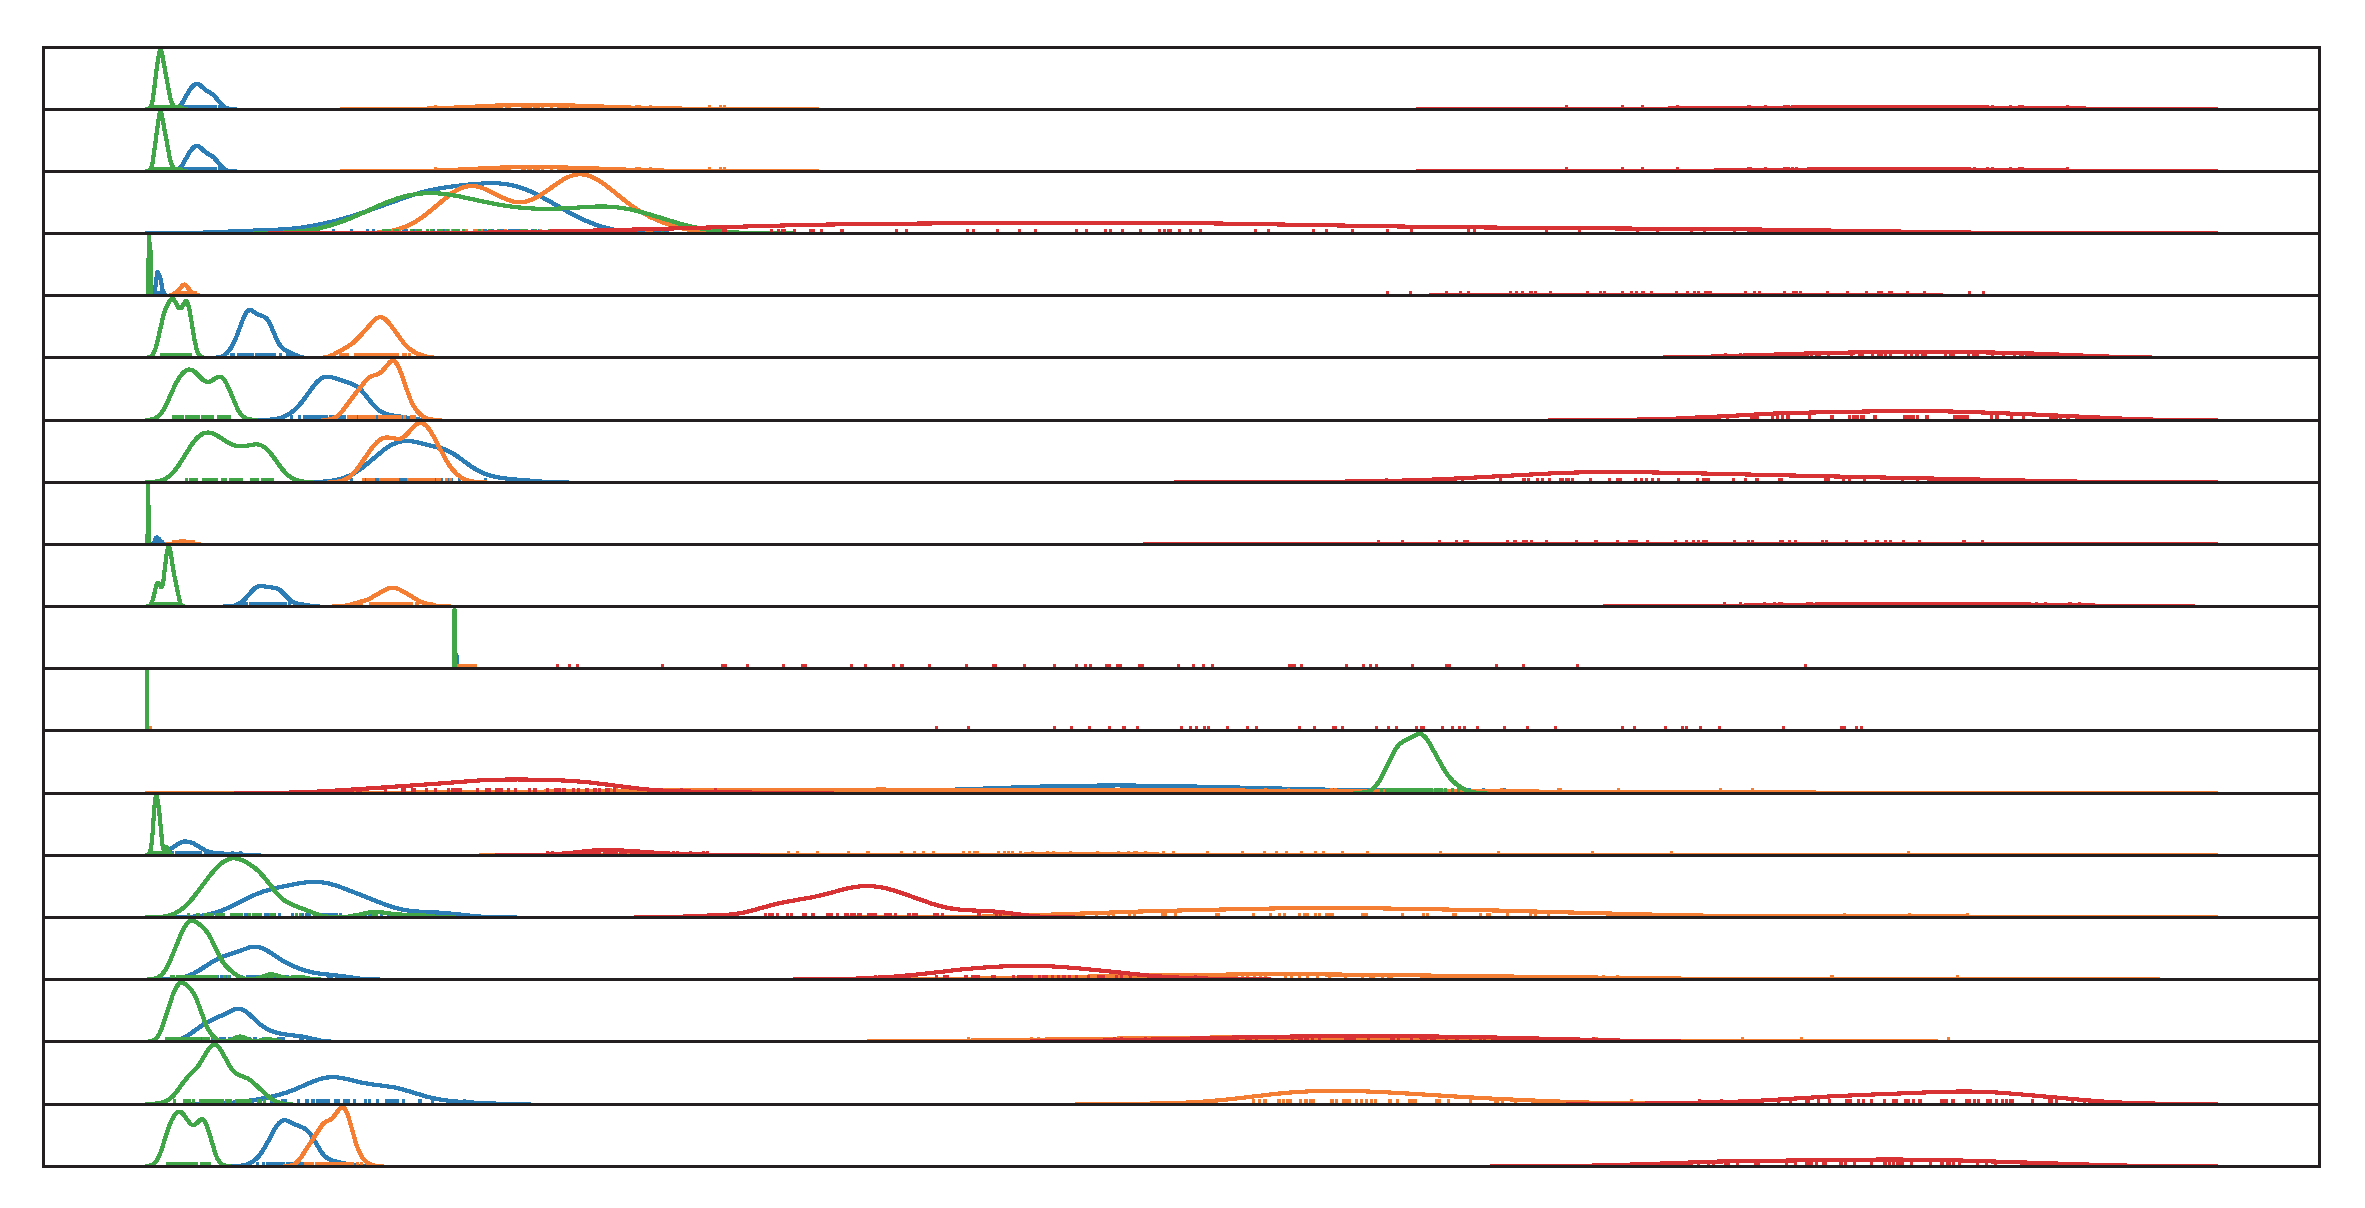
\includegraphics[width=\columnwidth]{feature.eps}
	\caption{The figure includes a total of 36 axes. In each axis, curves of different colors represent different fault type data.}
	\label{fig:feature}
\end{figure}

After the feature extraction, we can start the training of DBN. In this experiment, three RBMs are used, and the corresponding number of units per layer from bottom to top is 36, 18, 13, and 10. And we should add a classifier which has 10 units at the end of the DBN and compare the result with the label to determine the correctness. MomentumOptimizer is used in the back propagation. For each specific method, we run 50 times and average them for comparison. In the next three comparisons, the black curves always represents the method with theoretically better performance.

\subsection{DBN}
First we compare the differences between DBN and traditional back propagation neural network. As we can see from Fig. \ref{fig:dbnVSbp}, there was no significant improvement in the accuracy rate of the back propagation neural network in the first 200 epoches. The accuracy rate is about the accuracy rate at random selection, i.e. 10\%. 

When using DBN for the training, the initial accuracy rate can reach 20\%. And it converges faster, and the final accuracy rate is higher than the traditional back propagation neural network.

\begin{figure}[htbp]
	\centering
	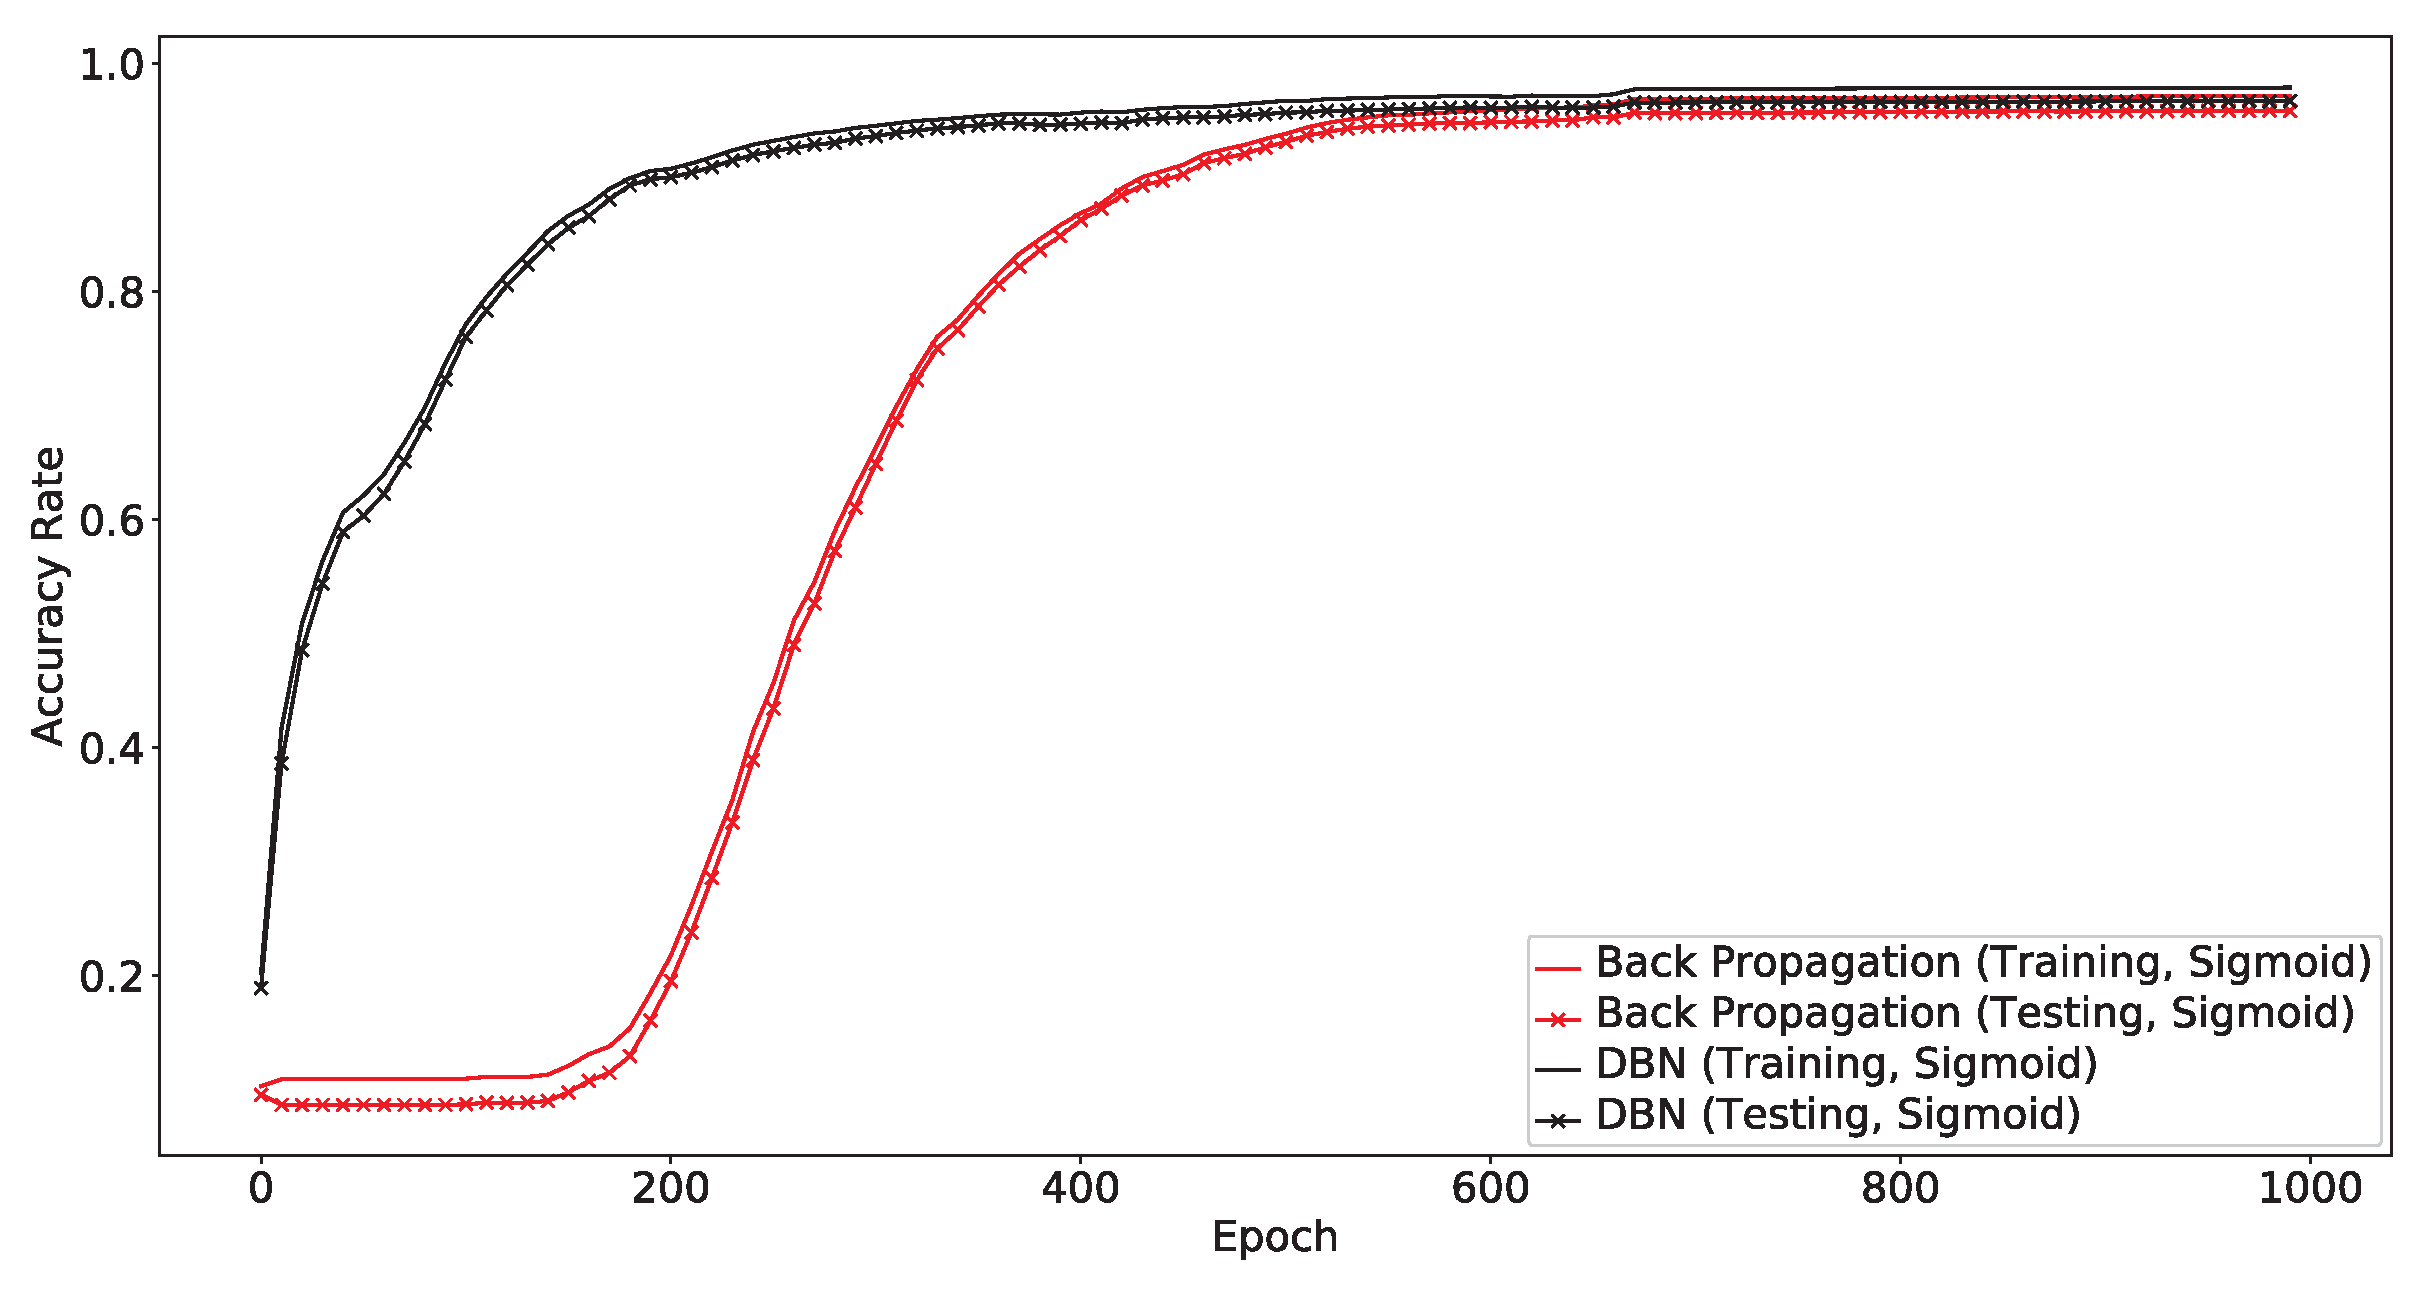
\includegraphics[width=\columnwidth]{dbnVSbp.eps}
	\caption{Comparison of classification accuracy between traditional back propagation neural network and DBN in 1000 epoches.}
	\label{fig:dbnVSbp}
\end{figure}

\subsection{Isigmoid}
Isigmoid proposed by Yi Qin \cite{YiThe} is capable to relax the vanishing gradient problem and converges faster then Sigmoid. As shown in Fig. \ref{fig:SigmoidVSIsigmoid}, since we did not use Isigmoid in RBM (pre-training), their initial accuracy rates are similar. However, when using Isigmoid in the back propagation, the DBN can converge faster and has higher accuracy rate.

\begin{figure}[htbp]
	\centering
	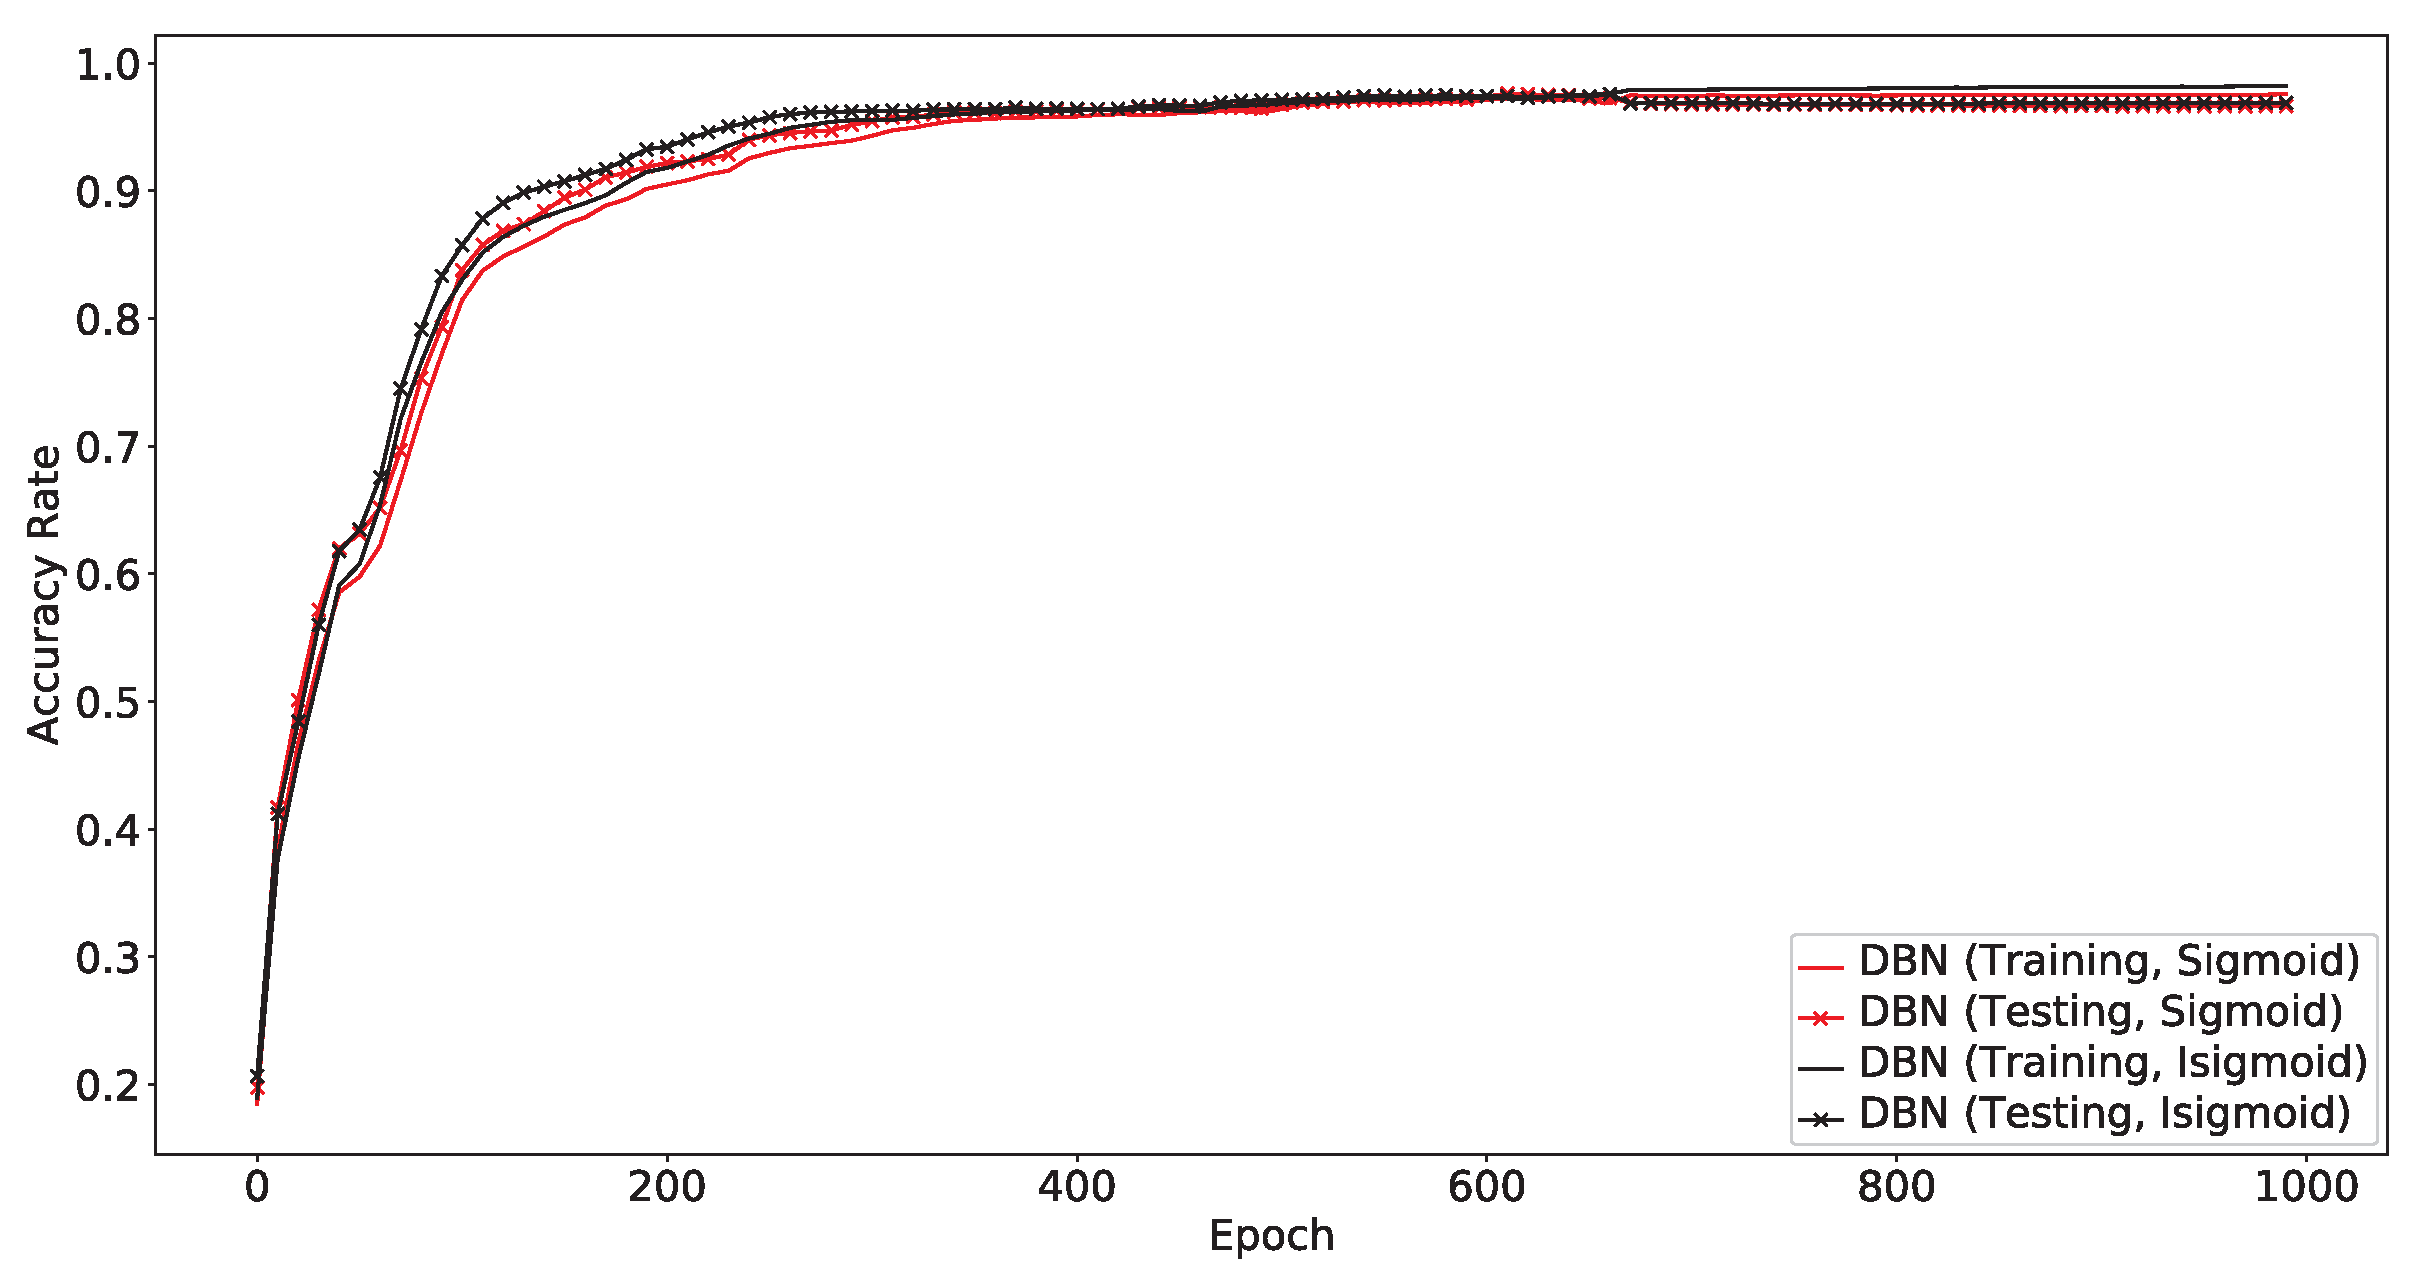
\includegraphics[width=\columnwidth]{SigmoidVSIsigmoid.eps}
	\caption{Comparison of classification accuracy between DBN using Sigmoid and DBN using Isigmoid in 1000 epoches.}
	\label{fig:SigmoidVSIsigmoid}
\end{figure}

\subsection{SSDBN}
\textcolor{red}{Next we compare DBN with SSDBN. Since SSDBN has studied the sample labels at RBM, I thought that the initial classification accuracy rate should be higher than DBN, but the result is not the case. And DBN seems to converge faseter than SSDBN. However, the final classification accuracy rate of SSDBN is higher than DBN.}

\begin{figure}[htbp]
	\centering
	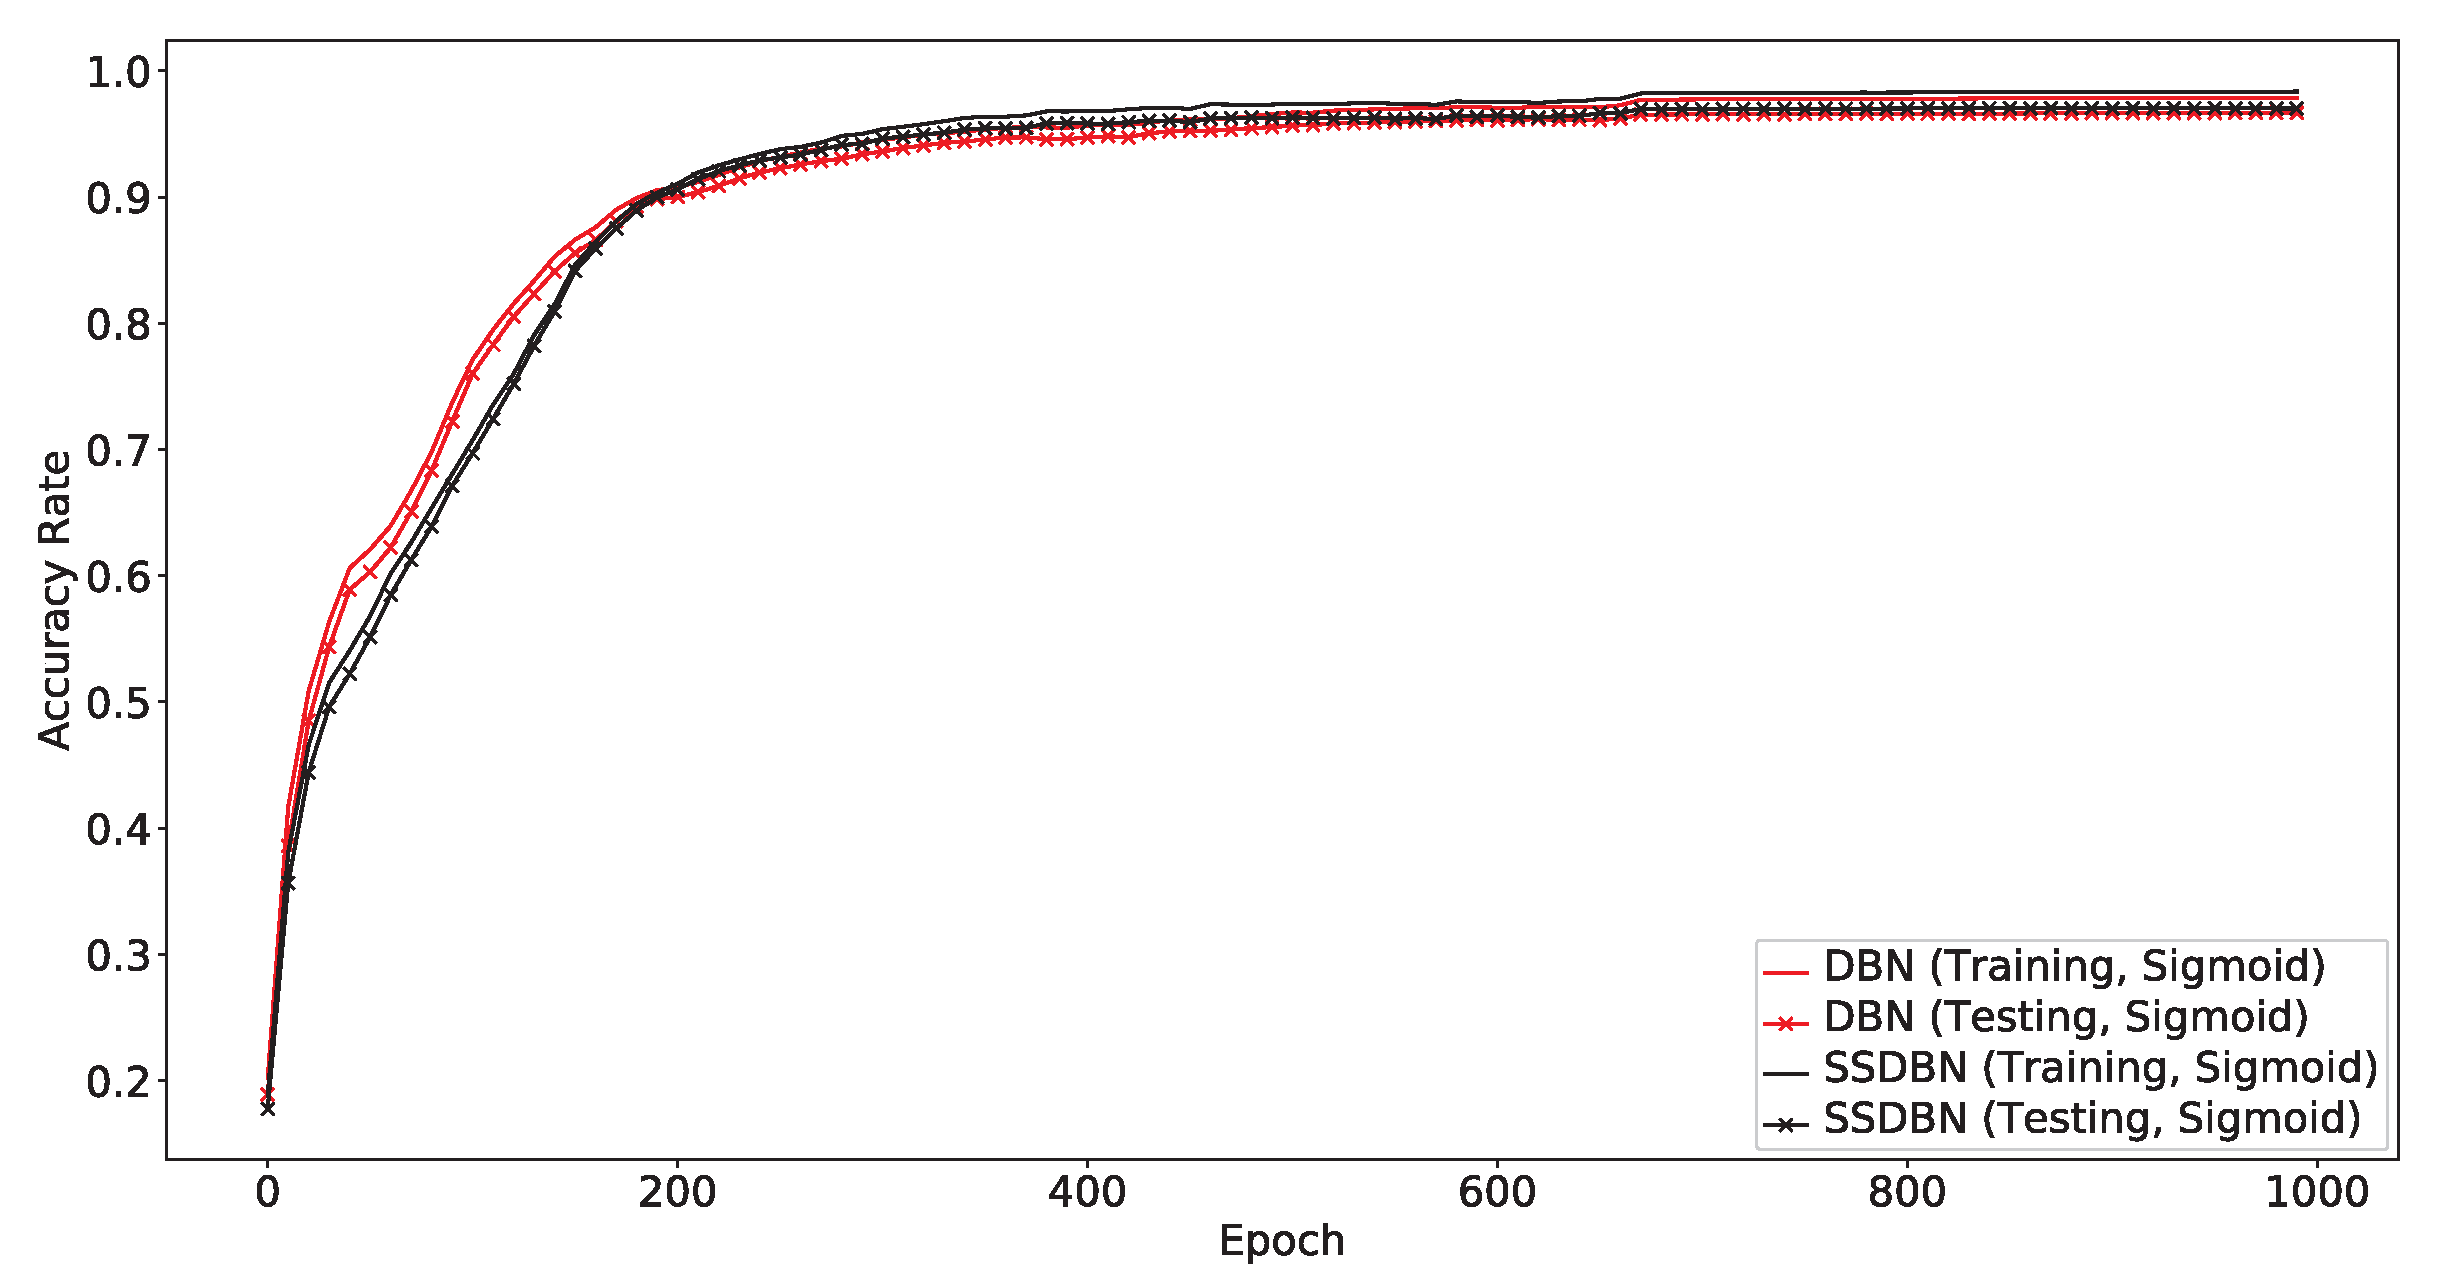
\includegraphics[width=\columnwidth]{SSDBN.eps}
	\caption{Comparison of classification accuracy between DBN and SSDBN in 1000 epoches.}
	\label{fig:SSDBN}
\end{figure}

In order to find out whether SSDBN really improves the performance of DBN, we compare the reconstruction error of each RBM. The reconstruction error can be calculated as 

\begin{equation}
R-Error = \sum_{s=1}^{N}\sum_{i=1}^{m}(v_{s,i}^{(0)}-v_{s,i}^{(1)})^2
\end{equation}
where $N$ is the number of input data and $m$ is the number of visible layer units.

The result is shown as Fig. \ref{fig:RBM012}. As we can see, in the first two RBMs, the SSRBM does reduce the reconstruction error.

\begin{figure}[htbp]
	\centering
	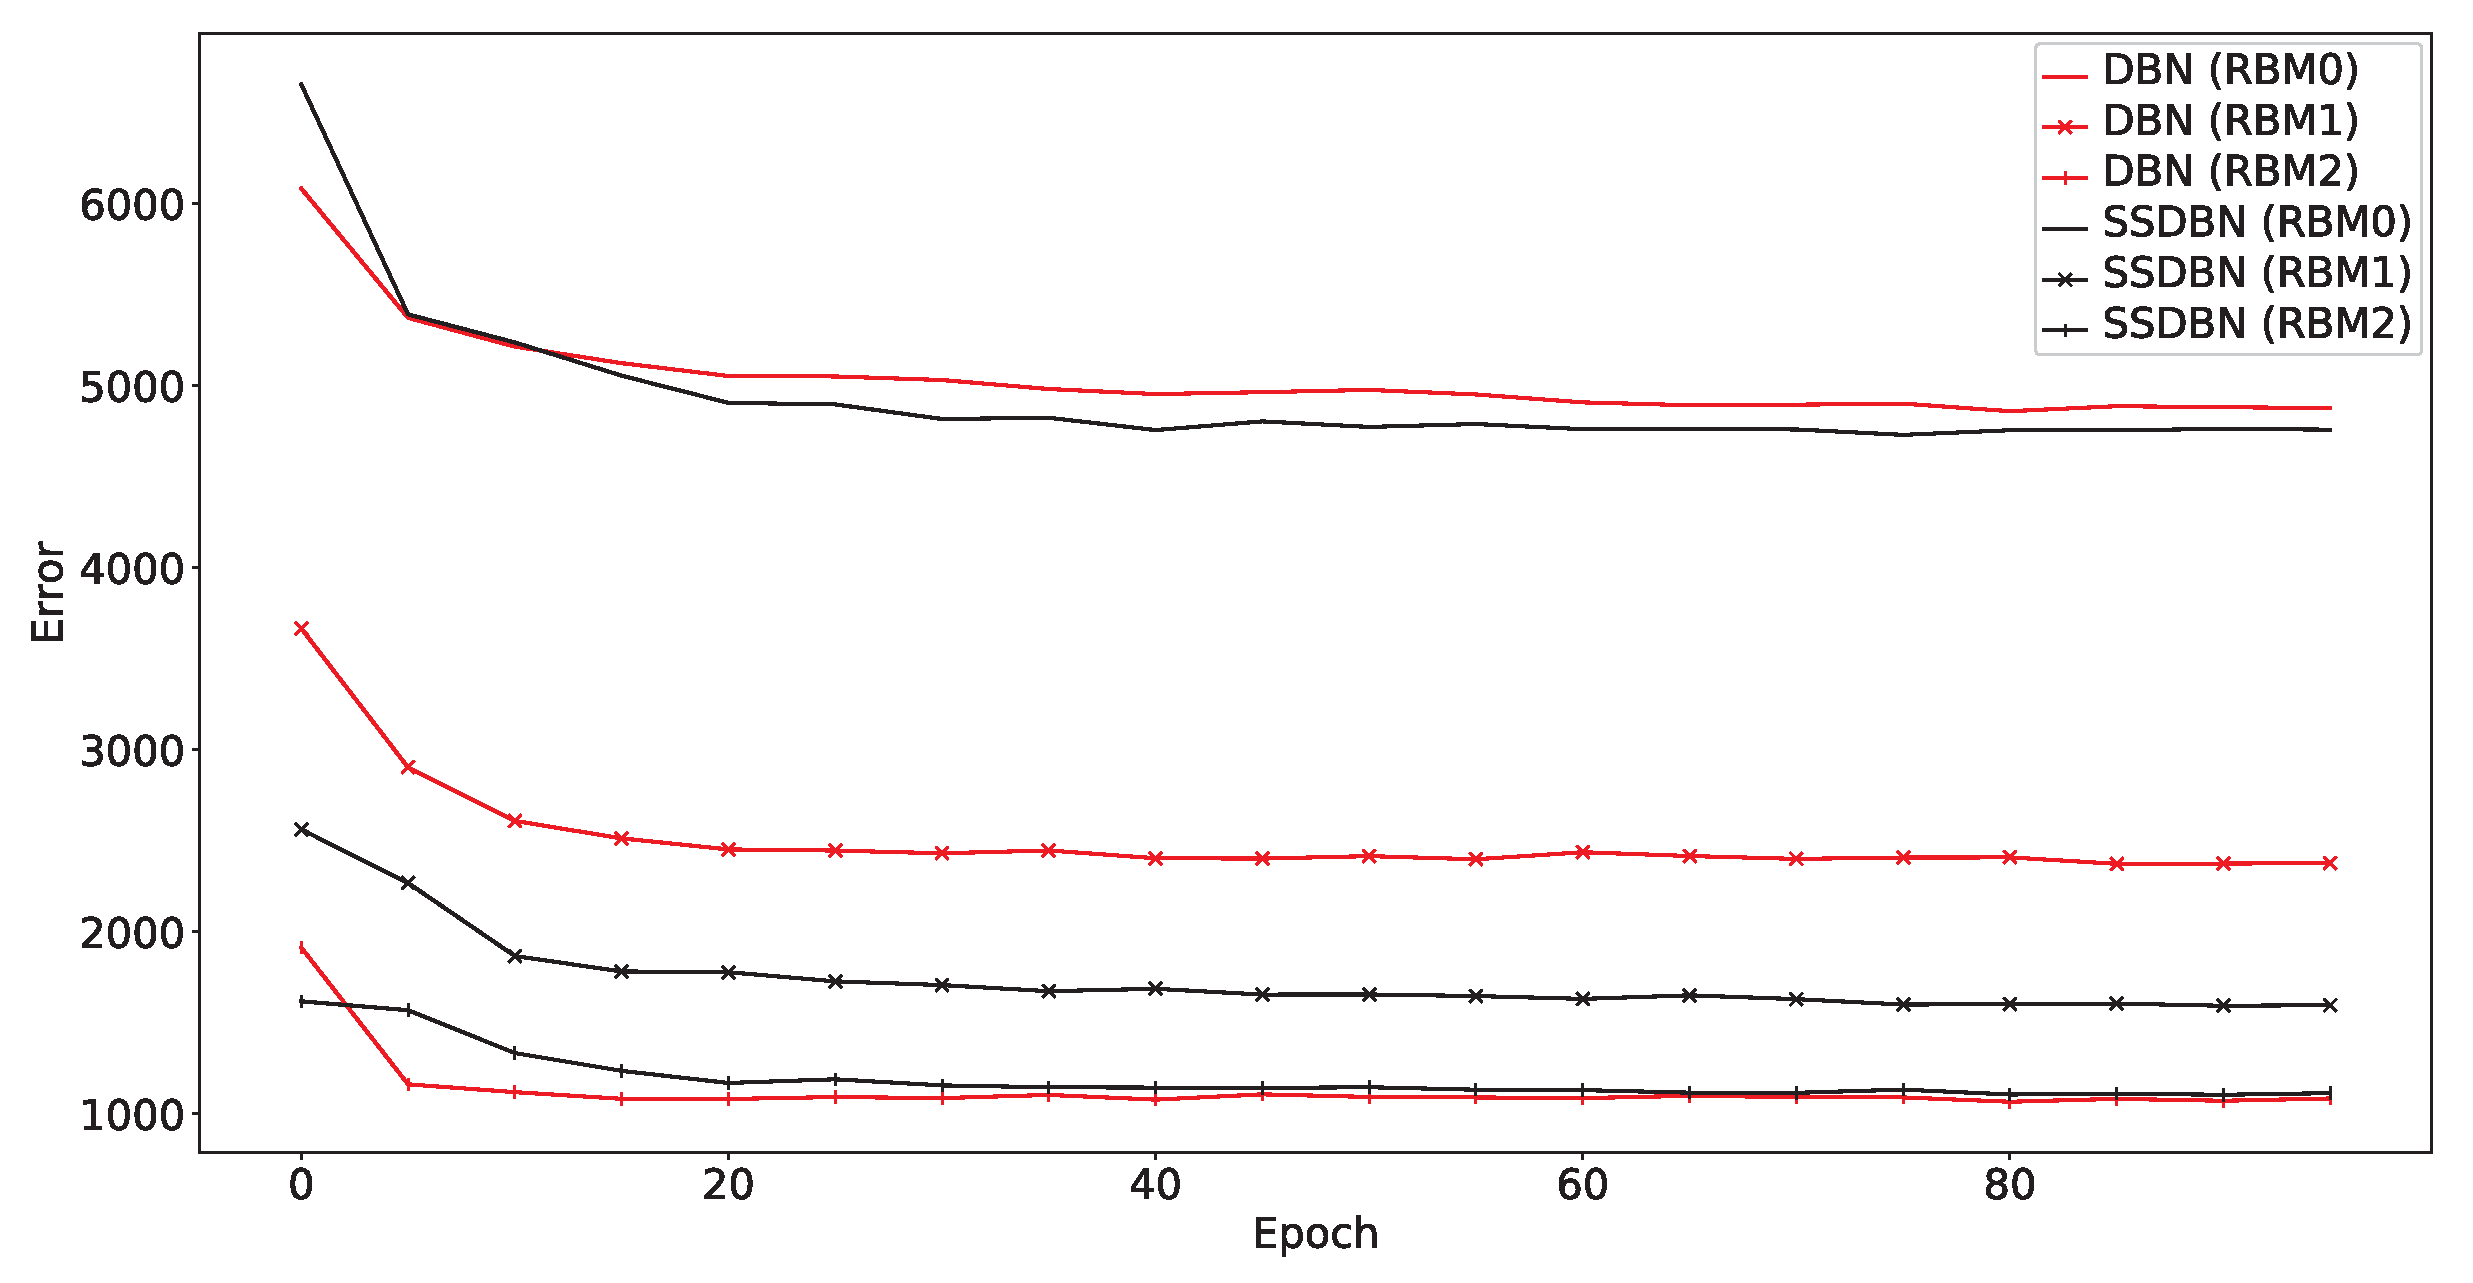
\includegraphics[width=\columnwidth]{RBM012.eps}
	\caption{Comparison of reconstruction error between DBN and SSDBN.}
	\label{fig:RBM012}
\end{figure}

Fig. \ref{fig:SSDBNIsigmoid} shows that by combining SSDBN with Isigmoid, we can further improve the classification accuracy.

\begin{figure}[htbp]
	\centering
	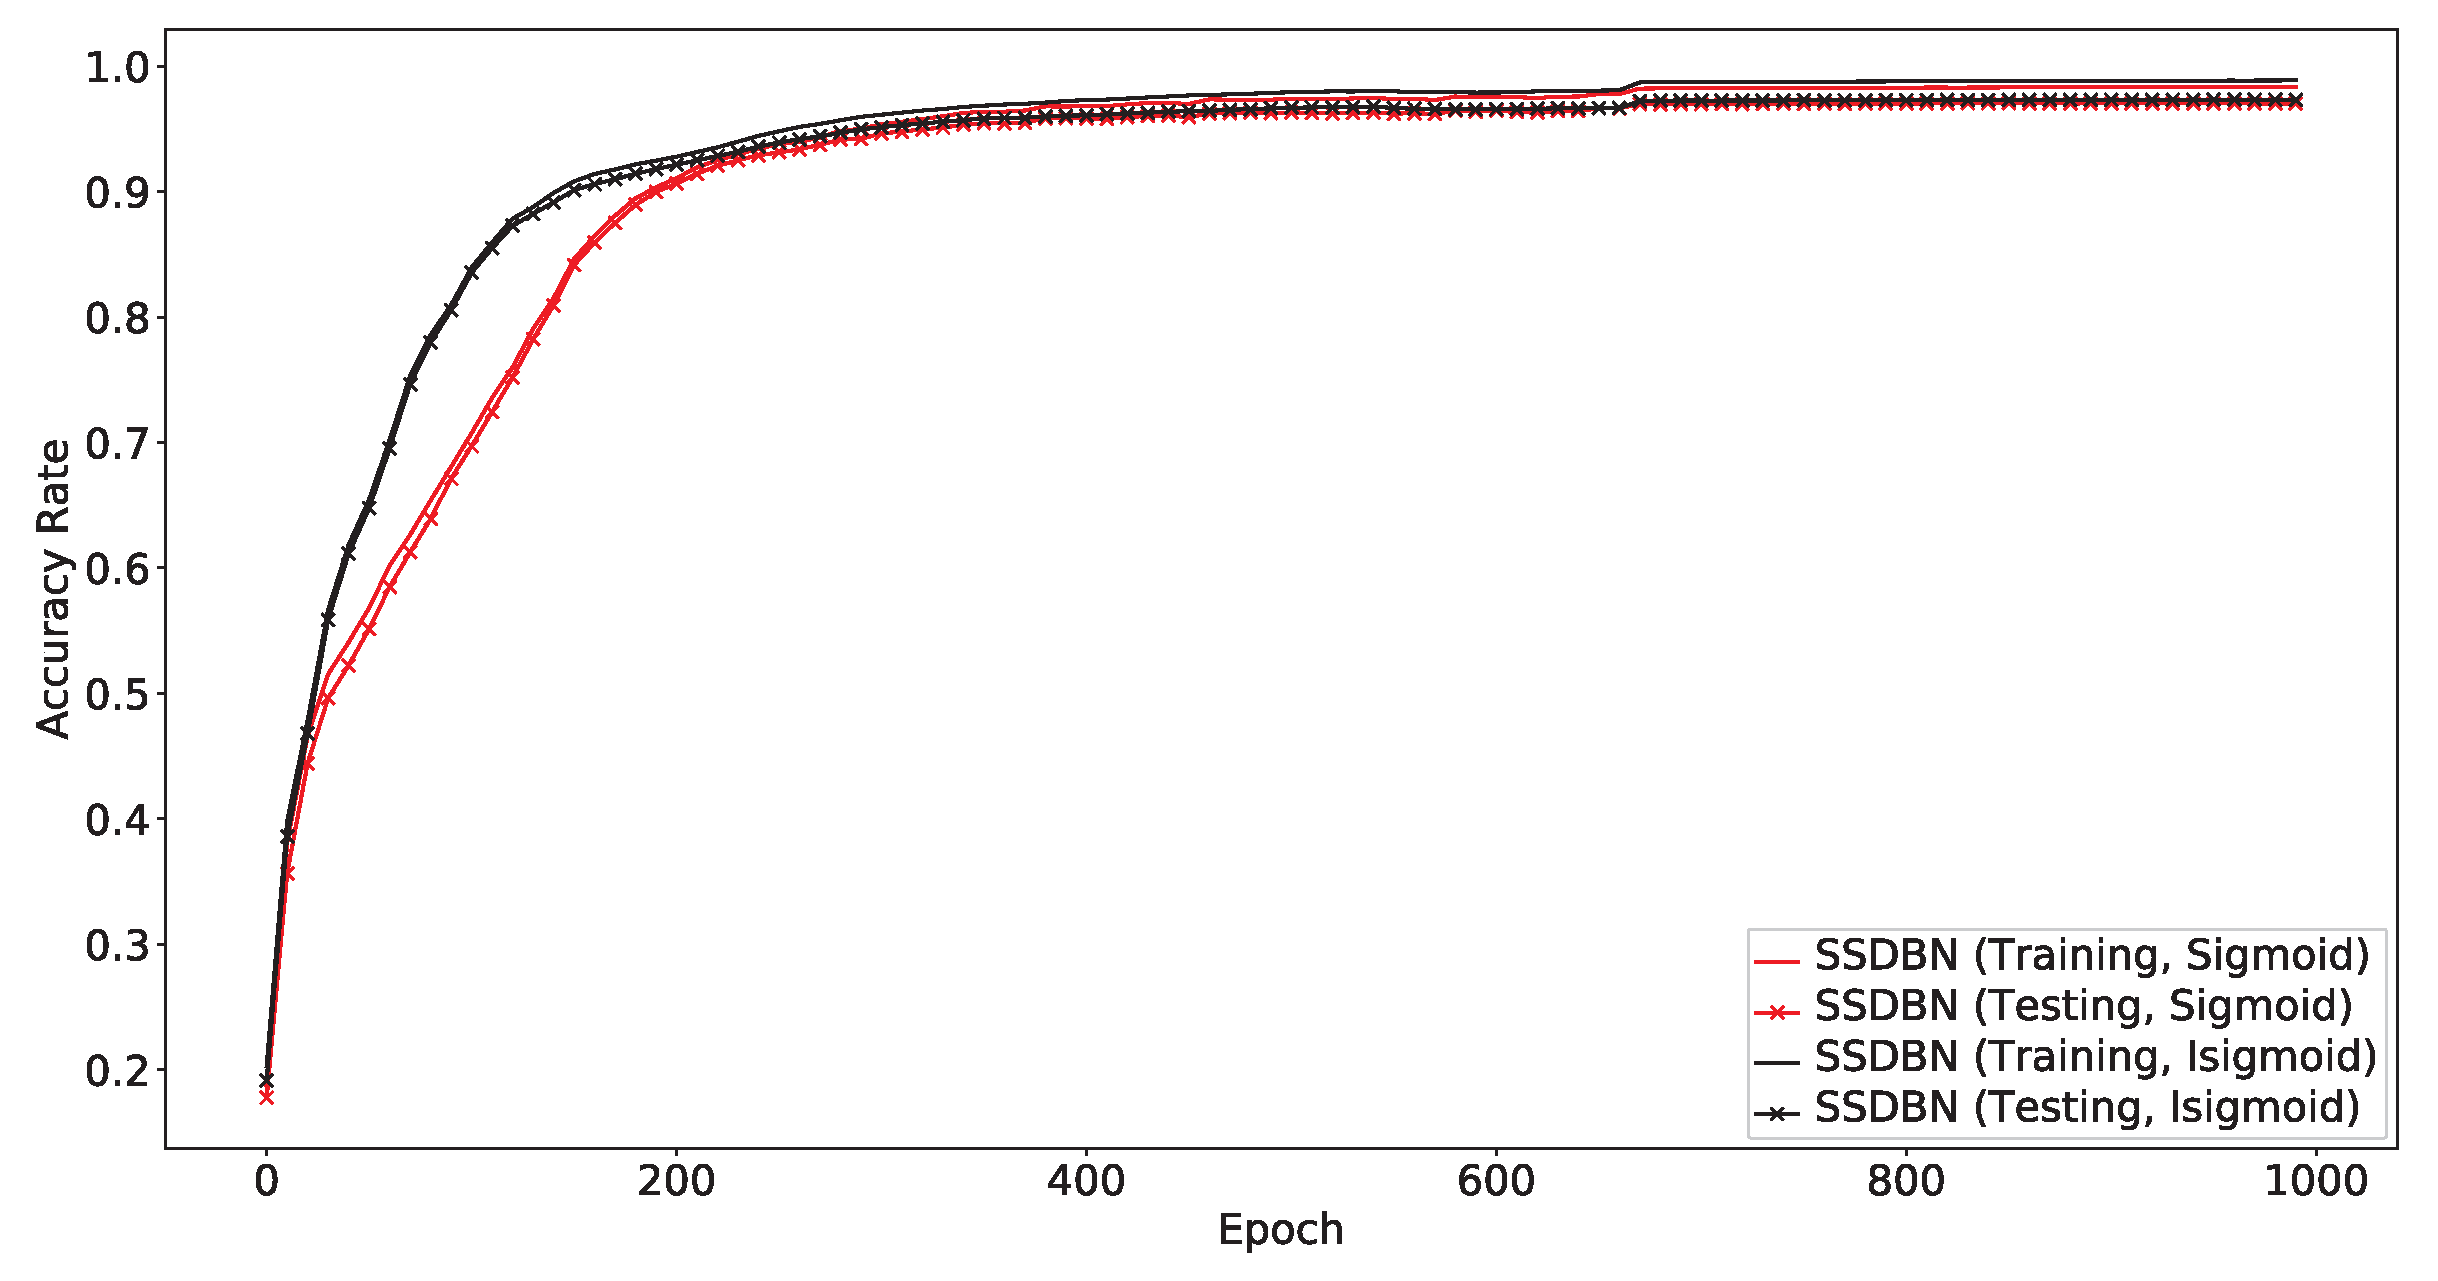
\includegraphics[width=\columnwidth]{SSDBNIsigmoid.eps}
	\caption{Comparison of classification accuracy between SSDBN using Sigmoid and SSDBN using Isigmoid in 1000 epoches.}
	\label{fig:SSDBNIsigmoid}
\end{figure}

In the traditional back propagation neural network, the accuracy rate of the training dataset is 97.12\%, and the accuracy rate of the testing dataset is 95.83\%. In the SSDBN using Isigmoid, the accuracy rate of the training dataset is 98.87\%, and the accuracy rate of the testing dataset is 97.33\%.

\section{Conclusions}
This paper is a summary of the project training. In this paper, two optimization methods of DBN are mainly involved, which are optimized from two aspects: activation function and structure. The paper also includes some noise reduction and feature extraction methods.

By using RBM, the DBN reduces the possibility of falling into the local minimum point due to the poor initial value when using the traditional back propagation neural network. The network after pre-training using RBM has better initial weight and bias, which makes neural network training more rapid, and has higher classification accuracy rate.

When using Sigmoid as the activation function, the problem of vanishing gradient easily occurs, and LReL cannot fully play its role in DBN. By combining them to form Isigmoid, the possibility of vanishing gradient problem is reduced, and the convergence is faster, and the advantages can be fully utilized in the DBN.

SSDBN optimizes the DBN structure and introduces semi-supervised learning into the DBN, which improves the classification accuracy. By combining SSDBN and Isigmoid, a higher classification accuracy rate can be achieved.

\textcolor{red}{Unfortunately, in this training, I have not come up with a better optimization method to improve the initial classification accuracy rate, speed up the convergence or improve the final classification accuracy rate. In addition, due to the lack of data and poor computer performance, I am unable to successfully train large data sets such as MNIST to further demonstrate the optimization effects of Isigmoid and SSDBN. At the same time, the parameter adjustment for each method may still cannot make the method achieve its optimal performance.}


\section*{Acknowledgement}
Acknowledgement is made for the measurements used in this work provided through data-acoustics.com Database. And I am grateful to senior apprentices and Ms. Huang for guiding me in the project training.



\bibliographystyle{unsrt}
\bibliography{ref} 


\end{document}
